\documentclass[journal]{IEEEtran}

% import graphics package to include images
\usepackage{graphicx}
\graphicspath{ {./images/} }
\DeclareGraphicsExtensions{.pdf,.jpeg,.png}

\usepackage{hyperref}
\usepackage{enumitem}
\usepackage{amsmath}
\usepackage{algorithm}
\usepackage[noend]{algpseudocode}
\usepackage{caption}

\begin{document}

% paper title
\title{Detecting Bots on Social Media}

% names of authors
\author{Manthan~Bharat~Bhatt, Simran~Singh}

% allocate space for title
\maketitle

% abstract of the report
\begin{abstract}
Social media forms an integral part of an average person’s life in today’s world. In the year 2017, the average daily social media usage of internet users was 135 minutes and is certain to increase perennially. While most content generated on these platforms is benign, automated computer programs, called bots, generate malicious information with varying degree of severity; from spam advertisements to bullying/threatening messages. This project aims to develop classification models to identify such malevolent computer programs on a social networking platform - Twitter and report efficiency of each model in terms of their Precision, Recall and F1 Score.
\end{abstract}

% indexing words
\begin{IEEEkeywords}
Bot Detection, Social Media, Twitter Data Analysis
\end{IEEEkeywords}

\section{Introduction}
\IEEEPARstart{T}{}witter has been one of the most used social media platform for over a decade now and this is largely due to its openness and minimalist behaviour. It allows its users to post micro blogs, usually about what is happening around them. The relationship between users in Twitter is directed; if user \textit{A} follows another user \textit{B}, then \textit{A} becomes a follower of \textit{B} and \textit{B} becomes a friend of \textit{A}. Users can decide whether they want to follow their friends back or not. The open nature of Twitter has led to creation of automated accounts called bots. These bots are created for wide range of applications - advertisements, recommendations, spreading news, spreading spam content etc. While some of the automated accounts are benign, most of them generate malicious content. The focus of this project is to detect such malicious bots and classify them into two categories - social bots and spam bots. Social bots are used to generate content in order to influence the views and actions of people. Such bots are extensively used during election campaigns. Spam bots on the other hand spread malicious, usually for phishing. In this project, we have successfully trained multiple supervised classifiers that can detect bots from both these classes. We have fine-tuned each classifier's hyper-parameters and made a comparative analysis based on a few matrix. However, getting labelled data is expensive and not always possible. Therefore, we also present some discriminating features that can be used to cluster un-labelled data into bots and non-bot accounts. 

The report is divided into seven sections. In section \RomanNumeralCaps{2}, we discuss some important terminologies that are essential for understanding the content of this report. Following that, section\RomanNumeralCaps{3} describes the data-set used and section \RomanNumeralCaps{4} and \RomanNumeralCaps{5} discuss our experimentation and the results we achieved respectively. The challenges we faced and future scope of this work in listed in section \RomanNumeralCaps{6} and we conclude the report in section \RomanNumeralCaps{7}.


\section{Terminology}
Before we begin to describe our solution, it is important that the reader gets familiar with a few definitions. This section lists some background knowledge that will be required for complete understanding of the report.


\begin{enumerate}
    \item Decision Trees: Decision trees are currently one of the most popular methods used for data modelling. They have the advantage of being conceptually simple, and have been shown to perform well on a variety of problems. Decision trees are constructed recursively from training data using a top-down greedy approach in which features are sequentially selected. During this feature selection process, the features that partition the set of instances into a more pure subset are preferred. The feature that has maximum information gain is said to be purest. 

	$$IG(A,S) = H(S) - \sum_A \frac{\left |S_v  \right | }{\left |S \right |} H(S_v)$$

    \item Random Forest: Random Forest is an ensemble learning method that classifies the data by constructing numerous decision trees while training and then producing the class which is mean of the individual decision trees. An ensemble learning algorithm work on the principal of training a set of "weak" learners and from these numerous weak training models build a "strong" model. The main advantage of using ensemble learning methods is to average out the outputs of individual weak learners, thus reducing the variance.   
    
    
    \item AdaBoost: AdaBoost is an acronym for Adaptive Boosting. It is also an ensemble learning method that learns sequentially i.e. the weights are adjusted giving more importance to miss-classified samples at each iteration. The algorithm for Adaboost Classification is given below:  

    \graphicspath{ {./images/} }
    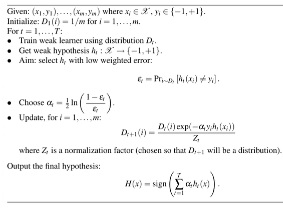
\includegraphics{adaboost_algo.jpg}
    
    
    \item Logistic Regression: Although the Logistic Regression has ‘regression’ in its name, it is a classification technique. It gets its name because it is very similar to linear regression, except the outcome is binomial. Some advantages of this model are analytical tractability and the ability to incorporate continuous valued features. The central mathematical concept that underlies logistic regression is the logit—the natural logarithm of an odds ratio. The simplest of models is of the form:

	$$logit(Y) = ln(odds) = ln(\prod/(1-\prod))$$

	Where Y is the posterior P(Y|X), which is the probability of having label Y after observing data X. 

    \item Support Vector Machines: Logistic Regression and Decision Trees fail in one aspect; they cannot construct complex decision boundaries. Support Vector Machines intend to overcome this very shortcoming. SVMs aim to find a hyper-plane $W^TX+b=0$ that best separates  the data. Here W is the vector of weights that is to be learned, X is the feature matrix and b is a bias. Solving for W and b results in a constrained Lagrangian optimization problem.


    \item K-Nearest Neighbor: KNN is a non-parametric learning algorithm that classifies the data by finding most similar k samples in the feature space. KNN is a lazy algorithm as there is no training process of the samples prior classification. As a result, KNN algorithm outputs higher accuracy for smaller data-sets. KNN finds the distance between the data-points for selecting the nearest neighbors. This distance can be measured using one of the following approaches: 
    \begin{enumerate}
        \item Euclidean Distance
        \item Manhattan Distance
        \item Camberra
    \end{enumerate}
\end{enumerate}

\section{Dataset}
We had applied for Twitter Developer API request quite sometime ago and have received it recently. Due to daily query limit, we have to rely upon alternate data sources. For this project, we have downloaded the data-set used by \cite{Data-Set}. The data-set contains account information for about 45000 users and 5 million tweets. Each user account is described by a set of 100 features and label that indicate the type of account (genuine user, social bot or spam bot). Our first challenge was to clean and transform this data in order to use it to train our models. The next step was to select features that had the maximum description and discrimination power. To this end, we took the following steps:
\begin{description}[font=$\bullet$]
	\item Each type of features - nominal, ordinal, ratio and interval were treated differently. Most of the nominal features were decriptive like tags or image summary. Such features were converted into a dictionary and feature vectors were created using their Tf-Idf weights. The numerical features were normalized (zero mean and 1 standard deviation) so that they all fall into similar range. For certain ordinal and interval features, a dictionary was created to convert them into numerical entities in order for classifiers to work better. For example, an ordinal feature have two values \textit{high} and \textit{low} can be converted into \textit{0} and \textit{1} respectively.
	\item Once the data was transformed, features with low entropy were dropped. Entropy describes the uncertainity of data and if a feature almost always has the same value irrespective of class label, it will not be a good classifier.
\end{description}


\section{Experimentation}

This section explains all the supervised classifiers we used and tuning of hyper-parameters for each algorithm to fit our use-case.

\begin{enumerate}

\item \textbf{Decision Tree and Random Forest}: For both these classifiers, we tuned the following parameters:
\begin{description}[font=$\bullet$]
\item criterion: When criterion was set as 'entropy', the accuracy was slightly higher than when it was set as 'gini'. This is observed because entropy is for attributes that occur in class and gini is for continuous attributes. In our data-set, we did not have many continuous attributes and as result 'entropy' performed slightly better. 
\item minimum sample leaf and minimum samples split - Reducing both the parameters slightly reduced the accuracy because if split samples is reduced there would be lesser number of purer nodes in the subsequent level of the decision tree. 
\end{description} 

\item \textbf{AdaBoost}: We tweaked the following parameters: 
\begin{description}[font=$\bullet$]
\item n estimators: We observed that higher the value of n estimators, better the accuracy would be because boosting is terminated at larger number of iterations. 
\item learning rate: As learning rate increases, the accuracy also increases. This observation was very intuitive. However, with a learning rate large enough, the classifier diverges.
\end{description}

\item \textbf{Logistic Regression}: Following parameters were tuned:
\begin{description}[font=$\bullet$]
\item max iters: When max iters was reduced, accuracy also went down because we forced the algorithm to converge faster that affected the accuracy. 
\item solver: We ran the algorithm with 'lbfgs' and 'newton-cg'. 'newton-cg' resulted in lower accuracy because for quadratic functions, newton-cg converges faster, whereas  L-BFGS converges slower. 
\end{description}

\item \textbf{Support Vector Machines}: Following parameters were tuned
\begin{description}[font=$\bullet$]
\item c: Changing the value of c had no effect on the accuracy of the system.
\item gamma: Increasing the value of gamma resulted in lower accuracy of the system because the radius of influence of the support vectors was very large that it only accommodated the support vector itself and no other sample. 
\end{description}

\item \textbf{KNN}: Following parameters were tuned:
\begin{description}[font=$\bullet$]
\item n-neighbors: Upon increasing the n-neighbors, the accuracy increased initially up to a certain point. But, after a certain increase in n-neighbours, the accuracy started dropping. 
\end{description}

\end{enumerate}

However, it is expensive to label data-points. Therefore, we also explored unsupervised learning algorithms to better understand ways in which bots can be identified if labels are not available. We first identified features that have the maximum entropy difference between bots and humans and then we ran K-Means clustering on those features. We present the results of our clustering next.

\begin{enumerate}
	\item The average tweet counts of humans vary by a large margin but they remain uniform for bots. Furthermore, the tweet counts for humans are much higher at the begining of the week and tend to decrease as the week progresses. This is not seen in bots however who post equally throughout the week
	\item The follower to friend ratio is almost equal to one more most users. In contrats, bots have a ratio close to zero. This happens because bots follow many users at a time but only a few users follow them back.
	\item Users are generally logged in at morning or at night. The activity of bots do not show any such pattern
\end{enumerate}

Through our analysis, we can say that tweet count, the days the tweets are posted, friends and followers count and login activity are good descriminators which can be used to cluster bots and humans if labelled data is not available


\section{Results}
We present the results we achieved in this section. We trained all the classifiers mentioned in the previous section and calculated classification accuracy, precision, recall and F1 scores on test set. 

\begin{center}
 \begin{tabular}{||c c c c c||} 
 \hline
 Classifier & Accuracy(\%) & Precision & Recall & F-1 \\ [0.5ex] 
 \hline\hline
 SVM & 42.94 & 0.32 & 0.43 & 0.43 \\ 
 \hline
 Random Forest & 32.91 & 0.63 & 0.43 & 0.58 \\
 \hline
 AdaBoost & 70.86 & 0.71 & 0.70 & 0.66 \\
 \hline
 Logistic Reg & 67.91 & 0.68 & 0.68 & 0.64 \\
 \hline
 Decision Tree & 59.41 & 0.59 & 0.58 & 0.54 \\
 \hline
 KNN& 62.74 & 0.61 & 0.64 & 0.57 \\ [1ex] 
 \hline
\end{tabular}
\end{center}


\section{Chanllenges}
We faced certain challenges while developing this solution. We decribe a few of those in this section. We believe these challanges my serve to be new directions of work in the field or help other researchers relate to our solution.

\begin{enumerate}
	\item \textbf{Cyborgs}\cite{Cyborg}: These are bots assisted humans or human assisted bots, i.e. a human with generates content with the help of a bot. It is difficult to detect cyborgs because they display the behaviour of both humans and bots. \cite{Cyborg} goes into details of detecting cyborgs but fails to attain satisfactory accuracy. One of the most commonly used method can be to classify accounts based on their tweet frequencies. Cyborg tweets are much more frequent and regular when compared to humans or classical bots.
	\item \textbf{Lack of Data}: Crawling data is a slow process, labelling it slower. This challenge can be countered by two methods - developing algorithms to self label the data or using efficient clustering algorithms to remove dependency on labels. We have experimented with a combination of both as explained in Section 4.
	\item \textbf{Changing Environments}: Trending topics on twitter change frequently which result in complete changes of bot behaviour. \cite{Dynamic-Bot} is a paper that explored into this to classify unlabelled data by running classifier on generated hidden features
\end{enumerate}

\section{Future Work}
This section lists a few directions that can be explored keeping this work as the starting point.
\begin{enumerate}
	\item \textbf{Using entropy of tweets to detect bots} \cite{Entropy}. This approach completely removes the requirement of procuring labelled data. \cite{Entropy} focuses frequency of tweets per week and calulates change in probability distribution every week. Humans generally have more erratic changes where bots have uniform distributions. However, this field is relatively unexplored and has extensive scope of research
	\item \textbf{Mitigating bot effect}. A lot of current research is on detecting bots but stopping their influence after detection is not focused much upon. 
\end{enumerate}

\section{Conclusion}
This project was a great learning experience for both of us. We learnt about various types of bots and their operating mechanisms. We also reliazed the positive and negative effects they can have on their environment. We then looked at various twitter data-sets and learnt what features can be significant to differentiate bots and humans. We gained deeper insights into a lot of supervised learning classifiers and learnt how to use them with our data. Lastly, we ackowledged the challenges we faced and identified interesting and significant research directions in the field.


\begin{thebibliography}{1}

\bibitem{Data-Set}
Cresci~S., Di~Pietro~R., Petrocchi~M., Spognardi~A. and Tesconi~M., \emph{The paradigm-shift of social spambots: Evidence, theories, and tools for the arms race}, \hskip 1em plus 0.5em minus 0.4em\relax in:\emph{Proceedings of the 26th International Conference on World Wide Web Companion (pp. 963-972). ACM}.

\bibitem{Dynamic-Bot}
Mehwish~Nasim, Andrew~Nguyen, Nick~Lothian, Robert~Cope and Lewis~Mitchell, \emph{Real-time Detection of Content Polluters in Partially Observable Twitter Networks} \hskip 1em plus 0.5em minus 0.4em\relax in: \emph{Companion Proceedings of the The Web Conference 2018, Pages 1331-1339}.

\bibitem{Cyborg}
Zi~Chu, Steven~Gianvecchio, Haining~Wang and Sushil~Jajodia \emph{Detecting Automation of Twitter Accounts: Are You a Human, Bot, or Cyborg?} in: \hskip 1em plus 0.5em minus 0.4em\relax \emph{IEEE TRANSACTIONS ON DEPENDABLE AND SECURE COMPUTING, VOL. 9,}

\bibitem{Entropy}
Rizal~Setya~PerdanaTri, Hadiah~MuliawatiReddy~Alexandro, HariantoReddy~Alexandro~Harianto \emph{Bot Spammer Detection in Twitter using Tweet Similarity and Time Interval Entropy}


\end{thebibliography}


\end{document}
